\documentclass{report}

\title{VSTTE'13 - DNS Server - Process, Requirements and Architecture}
\author{SPARK Pro-metheus Team}

\bibliographystyle{plain}

\usepackage[colorlinks=true,linkcolor=blue]{hyperref}
\usepackage{longtable}
\usepackage{array}
\usepackage{graphics}
\usepackage{xcolor}
\usepackage{rotating}
\usepackage{cite}

\usepackage{listings}
\lstdefinelanguage{SPARK}{
  language = [95]Ada,
  morekeywords = {pre,post,assert,assume,check,derives,hide,global,inherit,from,own,initializes,main_program},
  comment=[l][commentstyle]{--\ },
  texcl=true,
  showstringspaces=false
}

\lstdefinestyle{tinystyle}
   {basicstyle=\footnotesize\tt,
    keywordstyle=\color{blue},
    commentstyle=\rmfamily\it\color{gray},
    captionpos=b,
    caption={},label={},
    numbers=none,
    escapeinside={(*}{*)}}

\lstset{language=SPARK}
\lstset{style=tinystyle}


\usepackage{tikz}
\usetikzlibrary{calc,arrows,shapes,shadows,through}
\tikzstyle{main}=[regular polygon,
                  regular polygon sides=3,
                  draw,
                  minimum width=1cm,
                  inner sep=0.05cm,
                  text badly centered,
                  font=\scriptsize]
\tikzstyle{var}=[draw,
                 text badly centered,
                 text width=0.75cm,
                 font=\scriptsize]
\tikzstyle{type}=[rectangle,
                  draw,
                  rounded corners,
                  text width=0.75cm,
                  minimum height=0.5cm,
                  text badly centered,
                  font=\scriptsize]
\tikzstyle{boundary}=[single arrow,
                      draw,
                      shape border rotate=270,
                      single arrow head extend=0.0cm,
                      minimum height=0.75cm,
                      single arrow tip angle=120,
                      text badly centered,
                      text width=0.75cm,
                      font=\scriptsize]
\tikzstyle{utility}=[trapezium,
                     trapezium left angle=100,
                     trapezium right angle=100,
                     draw,
                     text width=0.75cm,
                     minimum height=0.5cm,
                     inner sep=0.01cm,
                     text badly centered,
                     font=\scriptsize]

\tikzstyle{strong}=[-triangle 90]
\tikzstyle{weak}=[-open triangle 90]


\usepackage[textsize=scriptsize,textwidth=4cm]{todonotes}
\newcommand{\mustDo}[1]{\todo[color=red!40]{MUST: #1}}
\newcommand{\shouldDo}[1]{\todo[color=orange!40]{SHOULD: #1}}
\newcommand{\mayDo}[1]{\todo[color=green!40]{MAY: #1}}
\newcommand{\thought}[1]{\todo[color=blue!40]{THOUGHT: #1}}
\newcommand{\questionDo}[1]{\todo[color=white!40,linecolor=black]{QUESTION: #1}}

\newcommand{\spark}[0]{{\sc Spark}}
\newcommand{\reveal}[0]{{\sc reveal}\texttrademark}
\newcommand{\informed}[0]{{\sc informed}}




\begin{document}

\maketitle
\tableofcontents

\chapter{Process}
\section{Introduction}
This document provides an overview of the process, tools and
techniques used to translate the requirements supplied as
part of the project brief into a detailed specification, design
and implementation.

The \reveal, \informed\ and \spark 2014 tools and techniques are
discussed, and a brief biography of the team members is also
documented within this report.

\section{Scope and caveats}
Due to the size of the problem and the short duration of the
competition, we have chosen to reduce scope for the challenge in order
to provide an answer to each of the point-scoring categories. In
particular we wish to address what we believe the overarching idea of
the competition is: to show a combination of processes that can be
used for the entire project lifecycle, resulting in high-quality
verified software. The scope has been reduced in the following areas:

\begin{itemize}
\item We have only used a process inspired by the \reveal\ and
  \informed\ process, briefly introduced in the sections to
  follow. Due to due to time and competition constraints we have
  omitted key steps, such as stake-holder interviews from these
  processes.

\item The domain analysis, requirements and architecture is performed
  on the whole of the problem; emphasising breadth not depth. In
  particular none of the above are \emph{complete}, and intended to
  only provide an illustration of the full process - however hopefully
  the difference between requirements, specification and domain
  knowledge has been clearly illustrated.

\item Design, implementation, validation, verification and
  traceability is performed on only sub-problem 1; emphasising depth
  and not breadth.
\end{itemize}


\section{Process Overview}
The swimlane diagram shown in Figure ~\ref{fig:the_process} on page
~\pageref{fig:the_process} has three classes of swimlane:

\begin{itemize}
\item Development Artefacts - these are items that are either consumed
  or generated by a process activity. This will include the solution
  to the problem, together with the design and test artefacts produced
  during the creation of the solution.

\item Development Activites - these are the tasks to be performed to
  address the development goals of the project. The development
  activities are split across swimlanes representing different Team
  Member rolls within the project:

  \begin{itemize}
  \item Requirements Engineer
  \item Development Engineer
  \item Test Engineer
  \end{itemize}

  The development steps in the swimlane diagram are part of the
  applied techniques listed below :

  \begin{itemize}
  \item \reveal\ - Development Context Diagram; Elicit Requirements;
    Boundary identification; Develop Project Data Model; Develop
    Domain, Specification, Requirements and Satisfaction Argument.

  \item \informed\ - Develop \informed\ Architecture; Apportion
    requirements to Architectural components; Develop UML Diagrams
    (Optional).

  \item \spark 2014 code development - Refine Specification statements
    based upon architectural structure; Develop Code, Statically
    Analyse Code; Develop High-Level Test Conditions; Develop AUnit
    High-Level Test Cases; Develop Module Test Conditions; Develop
    Module Tests and relevant stubs; Exceute Tests.
  \end{itemize}

  Prior to the execution of the project two activities have been
  applied, these are: Process Definition and Tool Selection.  Process
  design is applied to all our projects, and is tailored to select
  procedures and processes from a library of techniques, and is
  intended to produce an optimal mechanism to deliver the solution.

\item Infrastructure - identifies the tools used in the solution of
  the problem.
\end{itemize}

\begin{sidewaysfigure}[p]
  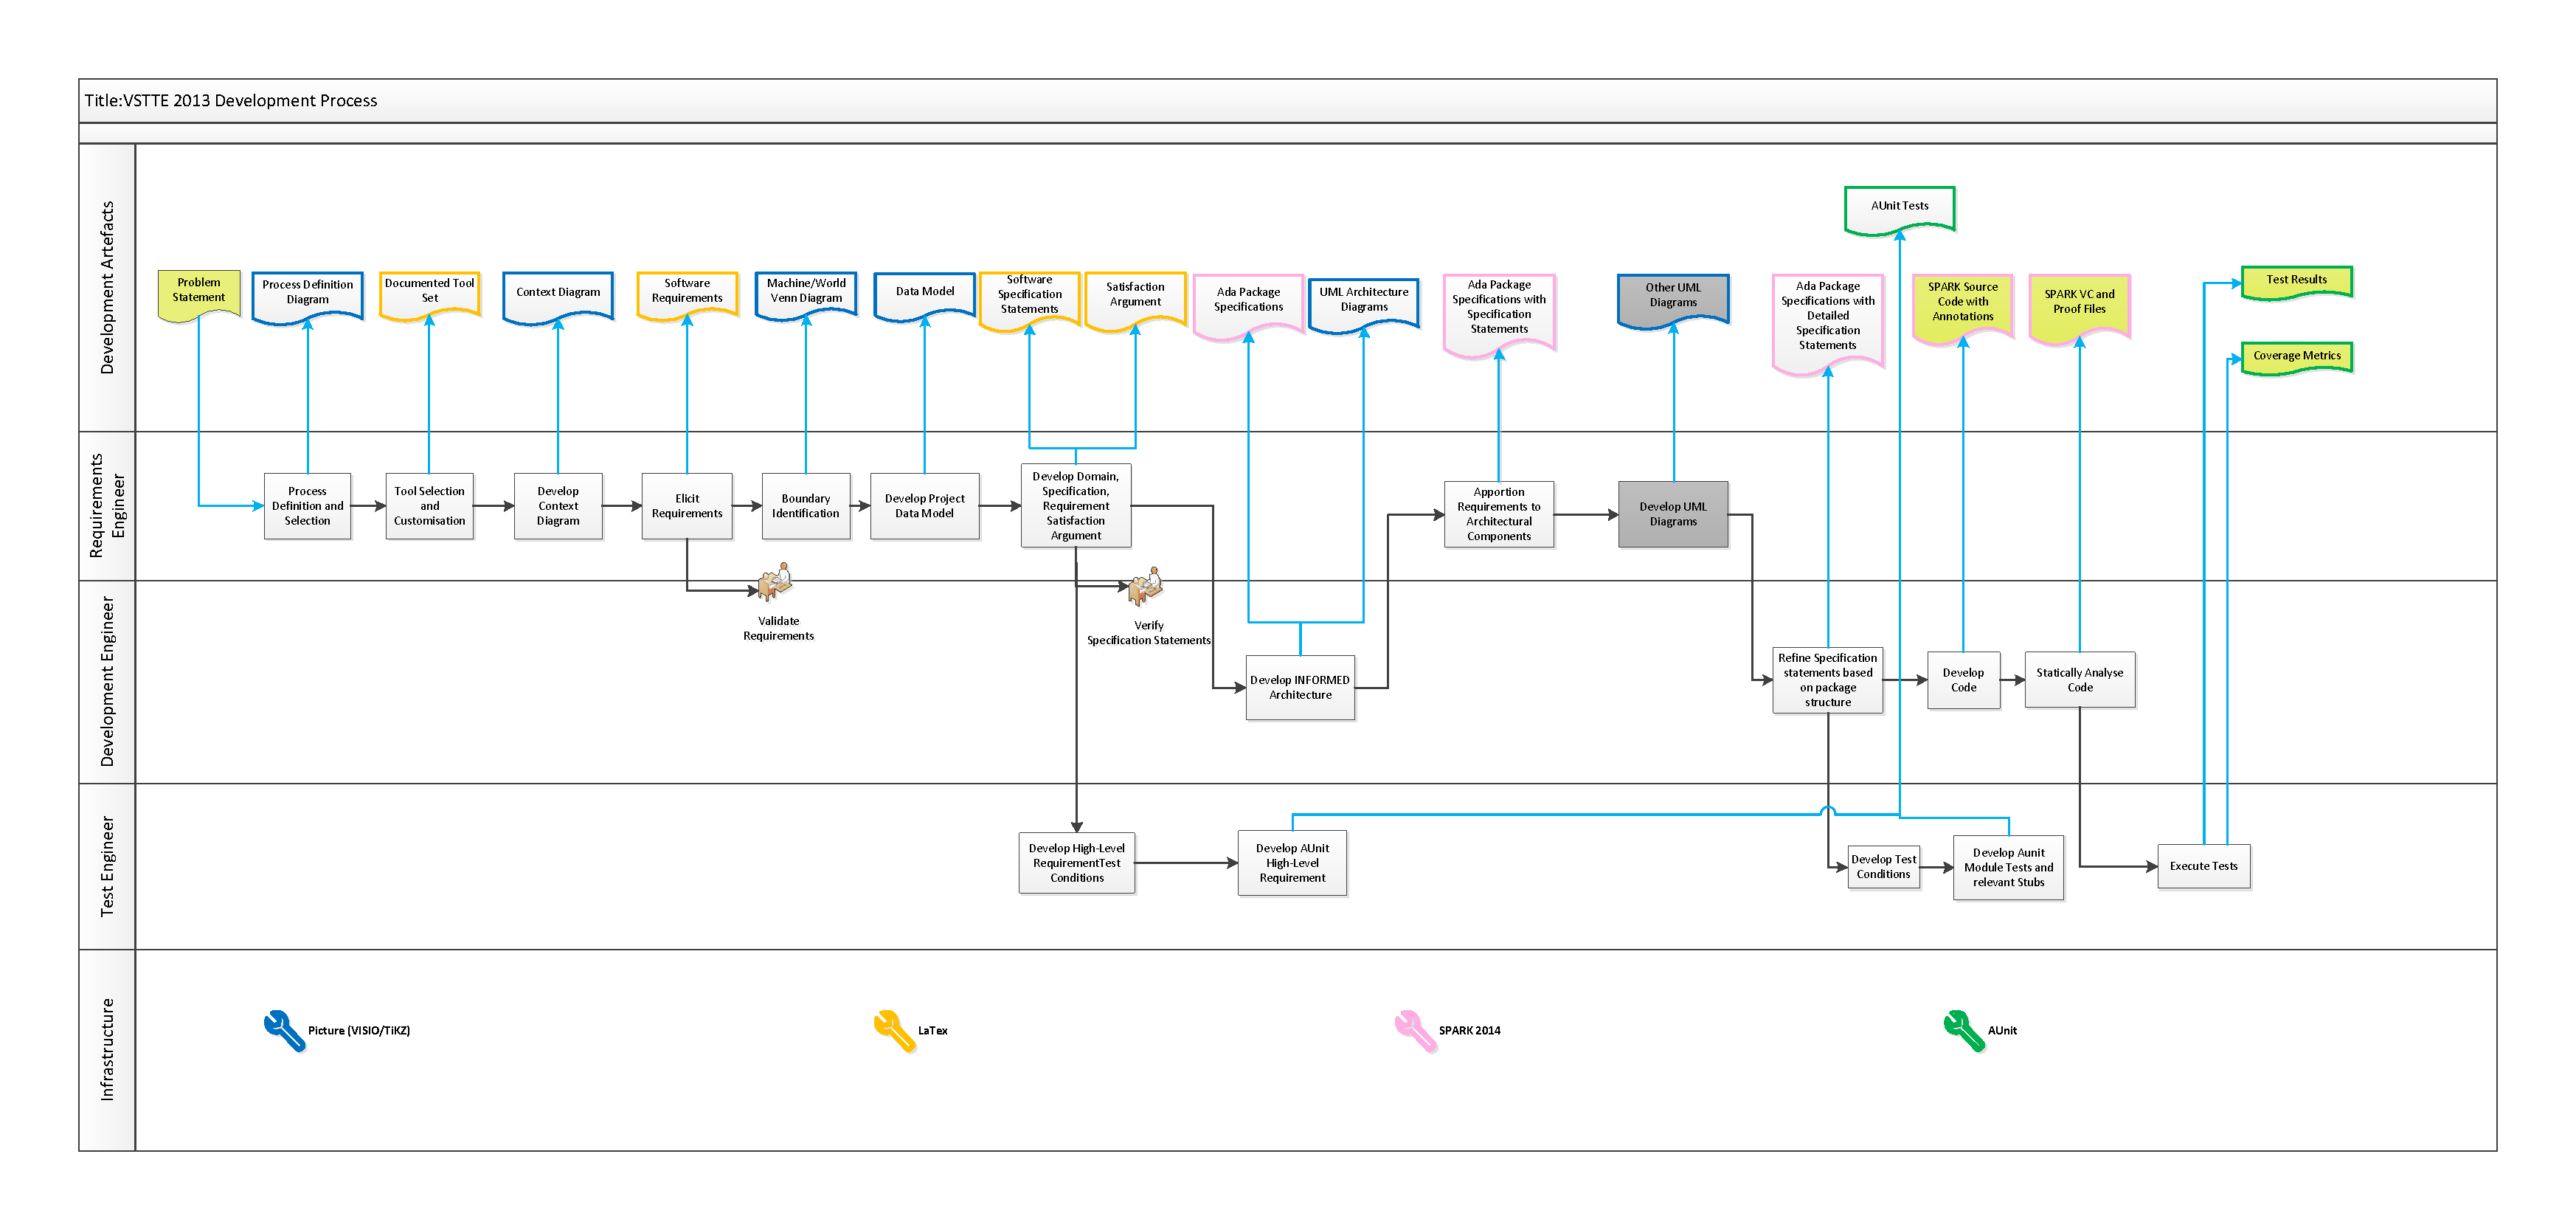
\includegraphics[width=\textwidth]{pictures/SwimLaneProcessDiagram.pdf}
  \caption{Our process for the VSTTE'13 competition}
  \label{fig:the_process}
\end{sidewaysfigure}

% Force swimlane diagram to appear in this section
\clearpage

\section{\reveal\ Overview}
\label{sec:reveal}
Software Engineering is concerned with the controlled and correct
development of Systems (Machines) that impact upon the environment in
which they are deployed (World). Where the objective of the deployment
of a Machine is to improve the World.

The purpose of Requirements Engineering is to take a set of
Stakeholder Requirements and arrive at a complete, correct and usable
set of System Specification Statements for the system under
development. Within \reveal\ the application of the
process is also intended to have a wider objective of adding benefits
to the project Stakeholders through learning, negotiation and the
development of trust between all parties involved in the production of
the system.

\reveal\ is Altrans' systematic method for the
elicitation, specification and management of System
Requirements. Through its application we clearly identify three key
artefacts:

\begin{itemize}
\item Requirements (R) which are statements about things in the World
  that we want the System to make true.

\item Specification Statements (S) describe the Systems external
  behaviour.
  \begin{itemize}
  \item Specifications include only shared phenomena in the interface
    between the World and the System being developed.
  \item Specifications can only constrain shared phenomena that the
    System can control.
  \end{itemize}

\item Domain Statements (D) which are knowledge about the World, that
  is generally assumed and not normally documented, but must hold if
  the Specification Statements are to fully satisfy the System
  Requirements.
\end{itemize}

\noindent
Once this information has been gathered, a Satisfaction Argument is
constructed to show that all the Stakeholder Requirements have been
addressed through the System Specification and Domain Statements. (As
Verification and Validation progresses, V\&V Plans and summary results
can also inform the satisfaction argument, although this may not be
done for the competition.)

The \reveal\ process is far more extensive than that described above
including detailed processes for:

\begin{itemize}
\item Stakeholder Identification,
\item Knowledge Elicitation,
\item Requirement Verification and Validation,
\item Conflict Management and Resolution,
\item Requirements Maintenance and Management.
\end{itemize}

\noindent
More information on the \reveal\ method can be found on:
\begin{center}
  \scriptsize
  \url{http://intelligent-systems.altran.com/technologies/systems-engineering/revealtm.html}
\end{center}

\noindent
Since by its nature the VSTTE 2013 competition has a very short
timescale, and the Requirements are provided by the competition
organisers it is not expected that there would be time to apply a full
\reveal\ process, however the benefits of Requirements capture,
expression, satisfaction arguments and traceability can be shown by
their application in this context.

\section{\informed\ Overview}
\label{sec:informed}
\informed\ is the Altran method for the construction of high-quality
software at a low-cost, it uses elements of both object oriented (OOD)
and functional design. OOD is used to establish the architecture of
the system and the elements of system state it contains. The result is
an annotated framework of \spark\ packages, constructing an architecture
that is modifiable and maintainable, which is capable of being
analysed at an early stage using the \spark\ tools.

Altrans' analysis of many software designs has identified that there
are 3 key building blocks that are used repeatedly to build an
application. These building blocks are:

\begin{itemize}
\item A Main Program, that is the top level, entry point controlling
  the behaviour a system or sub-system.
\item Variable Packages, which are \spark\ packages containing
  persistent "state", and are equivalent to what is commonly called an
  object.
\item Type Packages, which define the name of a type, and the
  operations taht it supports.
\end{itemize}

\noindent
In addition to these packages, \informed\ also includes two other
types of packages:

\begin{itemize}
\item Utility Packages, which provide shared functionality. The need
  for utility packages arises when an operation is required which
  affects or uses more than one variable of type package.

\item Boundary Variable Packages, which are particular kinds of
  variable package which provides interfaces between the software
  functionality described by the \informed\ design and elements
  outside it with which it must communicate. Unlike other variable
  packages the variable within the package is a place holder
  representing the stream of data arriving from, or being sent to, the
  outside world rather than simply an abstract name for the internal
  state of the package.
\end{itemize}

\noindent
The \informed\ method consists of 6 steps, and these are:

\begin{enumerate}
\item Identification of the System boundary, inputs and outputs.
\item Identification of the \spark\ boundary.
\item Identification and localization of the system state.
\item Handling initalization of state.
\item Handling secondary requirements.
\item Implementing the internal behaviour of components.
\end{enumerate}

\noindent
The output of the \informed\ process is represented a collection of
design diagrams and a collection of well defined \spark\
specifications. A summary of the \informed\ graphical elements and
example representations are documented in Annex A of this document to
aid the reader in the understanding of the architectural design.

As the VSTTE 2013 competition has a very short timescale, it is not
expected that there is enough time to fully apply the \informed\
process, however the benefits of the benifits of the modelling
approach and the translation in \spark\ Package Specifications can be
shown in this project.

\section{Tools}

\subsection{\spark 2014}
\spark\ is one of the premier environments for industrial development
of critical software. It consists of an Ada-based programming and
specification language and associated verification tools that provide
support for compositional, software-contract based specification and
verification for both functional and information flow
properties. Since its inception over 20 years ago, continuous research
and development has enabled \spark\ to establish an enviable
industrial track-record in the development of the most safety and
security-critical systems.

The next version of \spark\ to be issued in 2014 aligns \spark\ with
Ada 2012, and adds a host of new features over \spark 2005. Contracts
are now expressed as aspects and not comments, the language subset has
been greatly extended and the contract language itself is richer as
well. In addition, contract semantics are unified between the logical
and executable views.

The GNAT compiler for Ada supports most of \spark\ 2014 constructs
already.  The accompanying formal verification tool GNATprove
(co-developed between AdaCore and Altran) is currently available as a
prototype.

\section{The Team}
\paragraph{Alan Newton}\label{AlanNewton} is a Senior Software Engineer
working for \altran\ in Bath. He has a PhD in Software Engineering,
and has experience throughout the lifecycle. Not only has he
experience in developing high-integrity software using Formal Methods
and SPARK, he has also developed novel tools and processes for the
effective deployment of software engineering activities.

In this project Alan has been involved in developing the processes,
applying the \reveal\ and \informed\ processes and developing
documentation to support the delivery of the project.

\paragraph{Yannick Moy}\label{YannickMoy}
is a senior engineer at AdaCore, working on static
analysis and formal verification tools for Ada and SPARK programs. He
previously worked on similar tools for C/C++ programs at PolySpace,
INRIA research labs, and Microsoft Research. Moy received a PhD in
formal program verification from Universit\'e Paris-Sud.

In this project, Yannick has been involved in developing formal
specifications, implementing code, and verifying (formally and by testing)
that the code matches the formal specifications.

\paragraph{David Mentr\' e}\label{DavidMentre} is a research engineer at
Mitsubishi Electric R\&D Centre Europe, working on the application of
formal methods to industrial product development. He received a PhD in
Computer Science from Rennes~1 University.

In this project, David has been involved in... FIXME


\section{Acknowledgements}
As can be seen from the Team section, the members of this team have
been drawn from AdaCore, Altran and Mitsubishi Electric, and we would
like to thank our employers for there support in our taking part in
this competition.

We would especially like to thank them for allowing us to explore and
use their tools and techniques to build a well-defined process for
application to this problem.




\chapter{Requirements, Domain and Specification}
\section{Context Diagram}
\begin{center}
  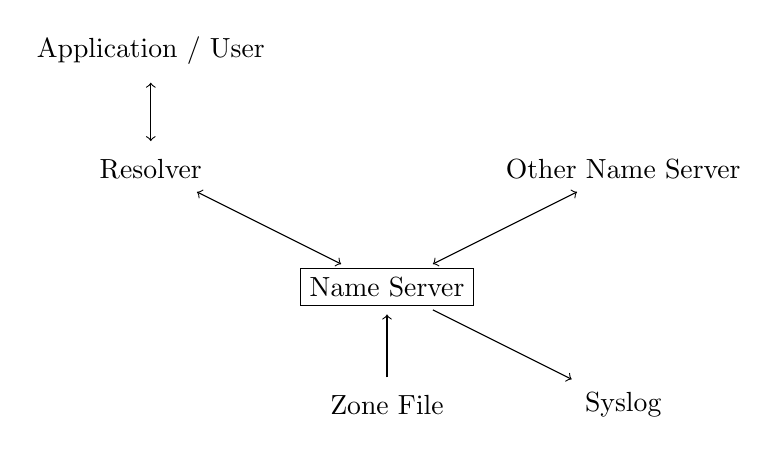
\begin{tikzpicture}[x=3cm,y=1.5cm,shorten >=3pt,shorten <=3pt]
    \node[draw] (dns) at (0, 0) {Name Server};
    \node (other_dns) at (1, 1) {Other Name Server};
    \node (zone_file) at (0, -1) {Zone File};
    \node (resolver) at (-1, 1) {Resolver};
    \node (user) at (-1, 2) {Application / User};
    \node (syslog) at (1, -1) {Syslog};

    \draw[<->] (user) -- (resolver);
    \draw[<->] (resolver) -- (dns);
    \draw[<->] (dns) -- (other_dns);
    \draw[->]  (dns) -- (syslog);
    \draw[->]  (zone_file) -- (dns);

  \end{tikzpicture}
\end{center}

\input{dsr/dsr.tex}
\input{dsr/dictionary.tex}


\chapter{Architecture}

\section{World-Machine Diagram}
\begin{center}
  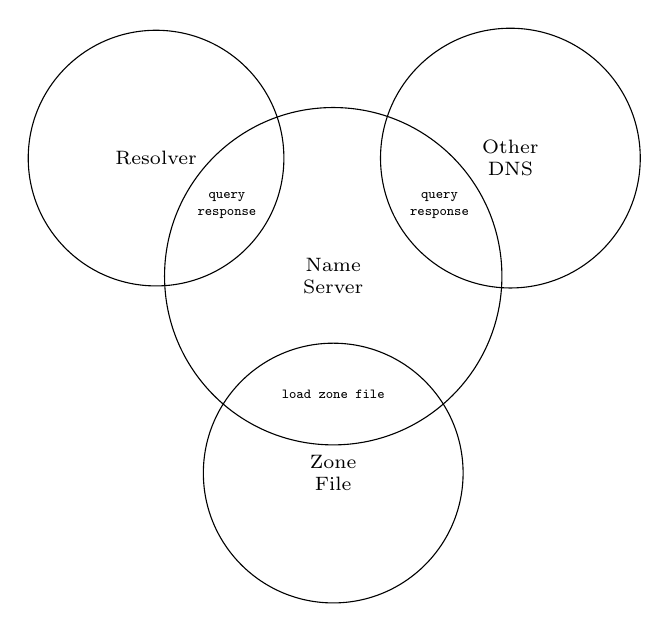
\begin{tikzpicture}[font=\scriptsize,x=1.5cm]
    \tikzstyle{circ}=[draw,circle,text width=3cm,text badly centered]
    \tikzstyle{lbl}=[text width=1.5cm,font=\tiny\tt,text badly centered]

    \node[circ,text width=4cm] at (0, 0) {Name\\Server};
    \node[circ] at (-1.5,  1.5) {Resolver};
    \node[circ] at ( 1.5,  1.5) {Other\\DNS};
    \node[circ] at (   0, -2.5) {Zone\\File};

    \node[lbl] at (-0.9,  0.9) {query\\response};
    \node[lbl] at ( 0.9,  0.9) {query\\response};
    \node[lbl] at ( 0.0, -1.5) {load zone file};
  \end{tikzpicture}
\end{center}

% \clearpage
% \section{\informed\ design}
% \begin{center}
%   \begin{tikzpicture}
%     \node[main] (main) at (0, 0) {main};

%     \node[type] (dns_t) at (-4, 1) {DNS\_T};
%     \node[boundary] (resolver) at (-4, -1) {Resolver};

%     \node[utility,text width=2cm] (dns_wfc) at (-3, 2) {DNS well-formed checker};
%     \node[utility,text width=2cm] (zd_wfc) at ( 0, 2) {Zone data well-formed checker};
%     \node[utility,text width=2cm] (parser) at ( 3, 2) {Zone file parser};

%     \node[boundary] (syslog) at ( 1.5, 4) {Syslog};
%   \end{tikzpicture}
% \end{center}

\bibliography{main}

\end{document}

